\documentclass{beamer}
\usepackage[utf8]{inputenc}
\usepackage{graphicx}
\usepackage{hyperref}
\usepackage{xcolor}

%tema + culoare
\usetheme{Singapore}
\usecolortheme{seahorse}
\setbeamertemplate{navigation symbols}{}

%info
\title{Descoperirea unui comutator molecular pentru 'vindecarea' celulelor canceroase}
\subtitle{O abordare revoluționară în tratamentul cancerului}
\author{Mara-Andreea Spataru}
\institute{Universitatea din București}
\date{26 Martie 2025}

\begin{document}
	
	%slide de titlu
	\begin{frame}
		\titlepage
	\end{frame}
	
	%slide de introducere
	\begin{frame}{Introducere}
		\begin{itemize}
			\item Tratamentele tradiționale ale cancerului se concentrează pe distrugerea celulelor canceroase
			\begin{itemize}
				\item Chimioterapie, radioterapie, imunoterapie
				\item Efecte secundare semnificative, distrugere și a țesuturilor sănătoase
			\end{itemize}
			\item Abordare nouă: inversarea celulelor canceroase în celule normale
			\begin{itemize}
				\item Nu distruge celulele, ci le transformă
				\item Potențial pentru mai puține efecte secundare
			\end{itemize}
			\item Echipa KAIST condusă de prof. Kwang-Hyun Cho a descoperit un \textbf{comutator molecular} pentru inversarea celulelor canceroase
		\end{itemize}
	\end{frame}
	
	%slide despre metoda de cercetare
	\begin{frame}{Fenomenul de tranziție critică}
		\begin{columns}
			\begin{column}{0.5\textwidth}
				\begin{itemize}
					\item Tranziția critică = schimbare bruscă de stare la un moment specific
					\begin{itemize}
						\item Similar cu transformarea apei în abur la 100°C
						\item La un punct specific, sistemul își schimbă radical comportamentul
					\end{itemize}
					\item Stare de tranziție instabilă:
					\begin{itemize}
						\item Coexistă caracteristici ale celulelor normale și canceroase
					\end{itemize}
					\item Moment crucial pentru intervenție terapeutică:
					\begin{itemize}
						\item Celula poate fi "împinsă" înapoi spre starea normală
					\end{itemize}
				\end{itemize}
			\end{column}
			\begin{column}{0.5\textwidth}
				\begin{center}
					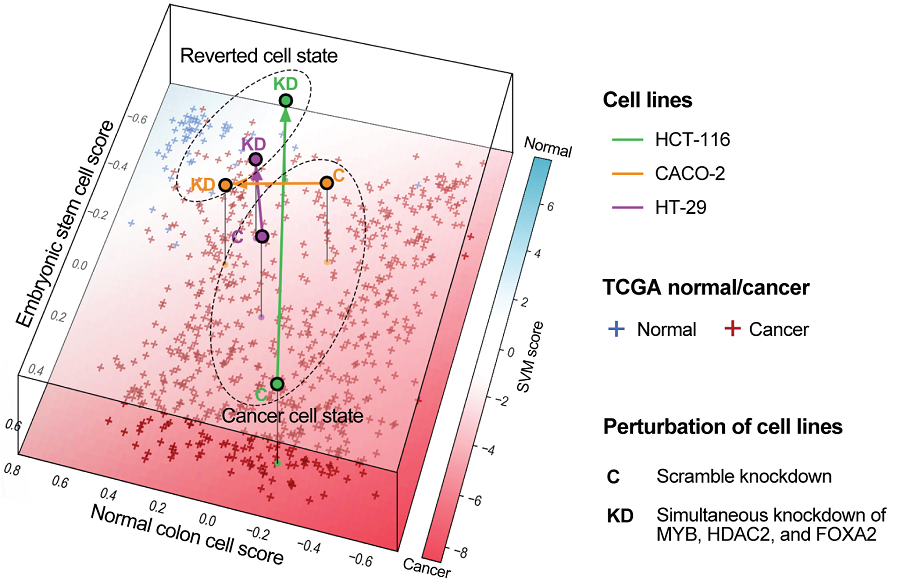
\includegraphics[width=\textwidth]{image1.png}
					
					\textbf{Reprezentare schematică a tranziției critice}
				\end{center}
			\end{column}
		\end{columns}
	\end{frame}
	
	%slide despre metodologia folosita
	\begin{frame}[allowframebreaks]{Metodologia de cercetare}
		\begin{itemize}
			\item Dezvoltarea unui model computerizat al rețelei genetice
			\begin{itemize}
				\item Tehnologie originală care construiește automat acest model
				\item Captează interacțiunile complexe dintre gene în timpul tranziției
			\end{itemize}
			\item Utilizarea datelor de secvențiere ARN la nivel de celulă unică
			\begin{itemize}
				\item Analiza expresiei genelor în fiecare celulă individual
				\item Identifică celulele aflate în starea de tranziție critică
			\end{itemize}
			\item Analiza sistemică pentru identificarea comutatoarelor moleculare
			\begin{itemize}
				\item Simulare și analiză computațională a modelului
				\item Identificarea punctelor cheie în rețeaua genetică (gene/proteine ce pot fi țintite)
			\end{itemize}
			\item Testare pe celule de cancer de colon
			\item Colaborare cu Universitatea Națională din Seul pentru organoide
			\begin{itemize}
				\item Organoide = țesuturi cultivate in vitro din pacienți cu cancer
			\end{itemize}
		\end{itemize}
		
		\framebreak
		
		%\begin{center}
			%\includegraphics[width=0.6\textwidth]{research_methodology.png}
			
			%\textbf{Fluxul de lucru pentru identificarea comutatoarelor moleculare}
		%\end{center}
	\end{frame}
	
	%slide despre rezultate
	\begin{frame}[allowframebreaks]{Rezultate și impactul cercetării}
		\begin{columns}
			\begin{column}{\textwidth}
				\begin{itemize}
					\item Confirmarea experimentală a posibilității de inversare a celulelor canceroase
					\begin{itemize}
						\item Celulele de cancer de colon au fost revertite spre caracteristici normale
						\item Demonstrarea viabilității conceptului de "inversare" în loc de "distrugere"
					\end{itemize}
					\item Găsirea căilor specifice prin care se formează cancerul
					\begin{itemize}
						\item Comutator molecular = "întrerupător" care poate fi activat/dezactivat
						\item Țintește puncte cheie care controlează transformarea celulelor
					\end{itemize}
					\item Prima demonstrație la nivel de rețea genetică a procesului de dezvoltare a cancerului
					\begin{itemize}
						\item Vizualizarea detaliilor procesului anterior considerat un "mister"
					\end{itemize}
				\end{itemize}
			\end{column}
		\end{columns}
		
		\framebreak
		
		\begin{columns}
			\begin{column}{0.6\textwidth}
				\begin{itemize}
					\item Bază pentru dezvoltarea de noi abordări terapeutice cu mai puține efecte secundare
					\begin{itemize}
						\item Tratamente care vizează specific moleculele implicate în tranziție
						\item Evitarea efectelor sistemice ale chimioterapiei tradiționale
					\end{itemize}
				\end{itemize}
			\end{column}
			\begin{column}{0.4\textwidth}
				\begin{center}
					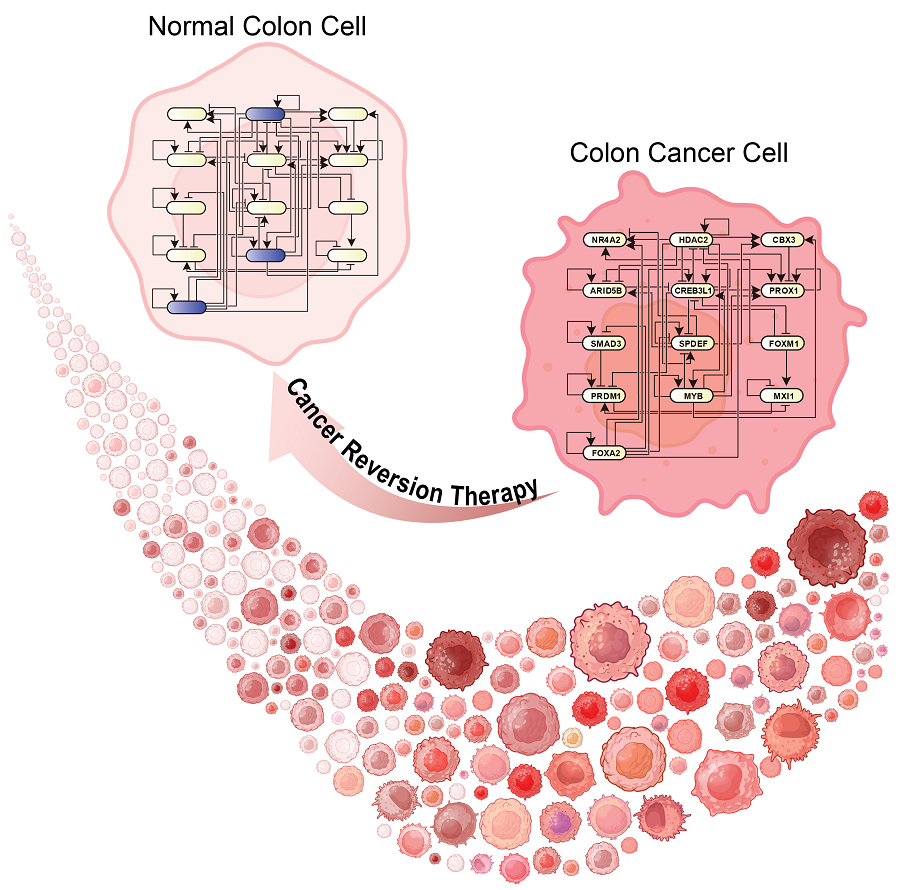
\includegraphics[width=\textwidth]{image2.png}
					
					\textbf{Procesul de inversare a celulelor canceroase}
				\end{center}
			\end{column}
		\end{columns}
	\end{frame}

	
	%slide de concluzie
	\begin{frame}{Concluzie}
		\begin{itemize}
			\item Descoperirea comutatorului molecular pentru inversarea celulelor canceroase reprezintă un progres semnificativ
			\begin{itemize}
				\item Prima demonstrație a posibilității de inversare a celulelor canceroase la nivel molecular
				\item Validată experimental pe celule de cancer de colon
			\end{itemize}
			\item Oferă o nouă perspectivă asupra biologiei cancerului
			\begin{itemize}
				\item Cancerul ca o stare celulară potențial reversibilă
				\item Importanța stărilor de tranziție în procesul de tumorogeneză
			\end{itemize}
			\item Deschide calea pentru strategii terapeutice inovatoare
			\begin{itemize}
				\item Tratamente care vizează normalizarea și nu distrugerea celulelor
				\item Abordări mai precise, cu intervenții în puncte specifice ale rețelei genetice
			\end{itemize}
			\item Potențial de a îmbunătăți calitatea vieții pacienților cu cancer
			\item Exemplu remarcabil de aplicare a bioinformaticii și biologiei sistemice în oncologie
		\end{itemize}
	\end{frame}
	
	%slide referinte
	\begin{frame}{Referințe}
		\begin{thebibliography}{9}
			\bibitem{ref1}
			News Medical Life Sciences. (2025, February 6). 
			\newblock KAIST team discovers molecular switch to reverse cancer cells. 
			\newblock Retrieved from https://www.news-medical.net/news/20250206/KAIST-team-discovers-molecular-switch-to-reverse-cancer-cells.aspx
			
			\bibitem{ref2}
			KAIST. (2025, February). 
			\newblock Professor Kwang-Hyun Cho's Research Team Discovers a Molecular Switch that Can Reverse Cancer. 
			\newblock Retrieved from https://news.kaist.ac.kr/newsen/html/news/?mode=V\&mng\_no=42710
		\end{thebibliography}
	\end{frame}
	
\end{document}